% 	Name		:: 	sthlm Beamer Theme  HEAVILY based on the hsrmbeamer theme (Benjamin Weiss)
%	Author		:: 	Mark Hendry Olson (mark@hendryolson.com)
%	Created		::	2013-07-31
%	Updated		::	June 18, 2015 at 08:45
%	Version		:: 	1.0.2
%	Email		:: 	hendryolson@gmail.com
%	Website		:: 	http://v42.com
%
% 	License		:: 	This file may be distributed and/or modified under the
%                  	GNU Public License.
%
%	Description	::	This presentation is a demonstration of the sthlm beamer
%					theme, which is HEAVILY based on the HSRM beamer theme created by Benjamin Weiss
%					(benjamin.weiss@student.hs-rm.de), which can be found on GitHub
%					<https://github.com/hsrmbeamertheme/hsrmbeamertheme>.


%-=-=-=-=-=-=-=-=-=-=-=-=-=-=-=-=-=-=-=-=-=-=-=-=
%
%        LOADING DOCUMENT
%
%-=-=-=-=-=-=-=-=-=-=-=-=-=-=-=-=-=-=-=-=-=-=-=-=

\documentclass[newPxFont]{beamer}
\usetheme{sthlm}
%\usecolortheme{sthlmv42}

%-=-=-=-=-=-=-=-=-=-=-=-=-=-=-=-=-=-=-=-=-=-=-=-=
%        LOADING PACKAGES
%-=-=-=-=-=-=-=-=-=-=-=-=-=-=-=-=-=-=-=-=-=-=-=-=
\usepackage[utf8]{inputenc}
\usepackage[T1]{fontenc}

%\usepackage{chronology}
\usepackage{chronosys}
\usepackage{subfigure}

\newcommand{\tabitem}{%
  \usebeamertemplate{itemize item}\hspace*{\labelsep}}

%\renewcommand{\event}[3][e]{%
%  \pgfmathsetlength\xstop{(#2-\theyearstart)*\unit}%
%  \ifx #1e%
%    \draw[fill=black,draw=none,opacity=0.5]%
%      (\xstop, 0) circle (.2\unit)%
%      node[opacity=1,rotate=45,right=.2\unit] {#3};%
%  \else%
%    \pgfmathsetlength\xstart{(#1-\theyearstart)*\unit}%
%    \draw[fill=black,draw=none,opacity=0.5,rounded corners=.1\unit]%
%      (\xstart,-.1\unit) rectangle%
%      node[opacity=1,rotate=45,right=.2\unit] {#3} (\xstop,.1\unit);%
%  \fi}%

%-=-=-=-=-=-=-=-=-=-=-=-=-=-=-=-=-=-=-=-=-=-=-=-=
%        BEAMER OPTIONS
%-=-=-=-=-=-=-=-=-=-=-=-=-=-=-=-=-=-=-=-=-=-=-=-=

%\setbeameroption{show notes}

%-=-=-=-=-=-=-=-=-=-=-=-=-=-=-=-=-=-=-=-=-=-=-=-=
%
%	PRESENTATION INFORMATION
%
%-=-=-=-=-=-=-=-=-=-=-=-=-=-=-=-=-=-=-=-=-=-=-=-=

\title{A Great Green Wall social-ecological systems database}
\subtitle{A tool for researchers and managers}
%\date{\small{\jobname}}
%\date{\today}
\date{15 juin 2016}
\author{\texttt{ E. Delay}}
\institute{\textsc{Ohmi} Téssékéré - Sénégal\\
\textsc{Geolab}, Université de Clermont-Auvergne.}

\hypersetup{
pdfauthor = {E. DELAY},
pdfsubject = {Réseau OHM},
pdfkeywords = {grande muraille verte, ANR future Sahel},
pdfmoddate= {D:\pdfdate},
pdfcreator = {}
}

\begin{document}

%-=-=-=-=-=-=-=-=-=-=-=-=-=-=-=-=-=-=-=-=-=-=-=-=
%
%	TITLE PAGE
%
%-=-=-=-=-=-=-=-=-=-=-=-=-=-=-=-=-=-=-=-=-=-=-=-=

\maketitle

%\begin{frame}[plain]
%	\titlepage
%\end{frame}

%-=-=-=-=-=-=-=-=-=-=-=-=-=-=-=-=-=-=-=-=-=-=-=-=
%
%	TABLE OF CONTENTS: OVERVIEW
%
%-=-=-=-=-=-=-=-=-=-=-=-=-=-=-=-=-=-=-=-=-=-=-=-=
%\section*{Overview}
%\begin{frame}{Overview}
%% For longer presentations use hideallsubsections option
%\tableofcontents[hideallsubsections]
%\end{frame}

%-=-=-=-=-=-=-=-=-=-=-=-=-=-=-=-=-=-=-=-=-=-=-=-=
%	FRAME: INTRODUCTION
%-=-=-=-=-=-=-=-=-=-=-=-=-=-=-=-=-=-=-=-=-=-=-=-=

\section{Introduction}

%-=-=-=-=-=-=-=-=-=-=-=-=-=-=-=-=-=-=-=-=-=-=-=-=
%	FRAME: ANR framework in 4 wp
%-=-=-=-=-=-=-=-=-=-=-=-=-=-=-=-=-=-=-=-=-=-=-=-=
\begin{frame}[c]{The Great Green Wall}
\vspace{-1cm}
Yes the Green Great wall can be in China, by our sandybox is in Africa, where we work for the "Future Sahel" ANR project.
\begin{figure}
	\centering
	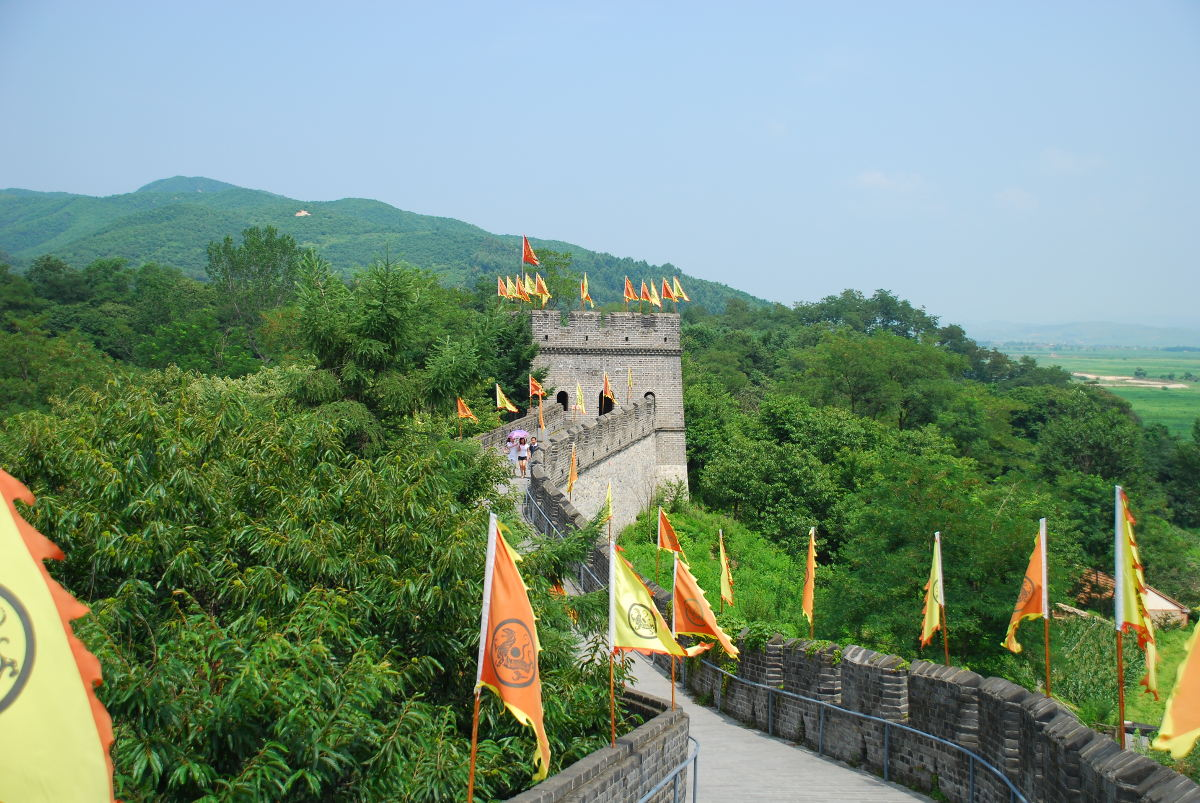
\includegraphics[width = 0.6\textwidth]{img/great_wall}
\end{figure}
\begin{center}
    \begin{tabular}{@{}l@{}}
       \\
      \tabitem width $\approx 15 km$ \\
      \tabitem length $\approx 7600km$
  \end{tabular}
\end{center}
\end{frame}

%-=-=-=-=-=-=-=-=-=-=-=-=-=-=-=-=-=-=-=-=-=-=-=-=
%	FRAME: ANR framework in 4 wp
%-=-=-=-=-=-=-=-=-=-=-=-=-=-=-=-=-=-=-=-=-=-=-=-=
\begin{frame}[c]{Future Sahel Framework}
\vspace{-1cm}
\begin{figure}
	\centering
	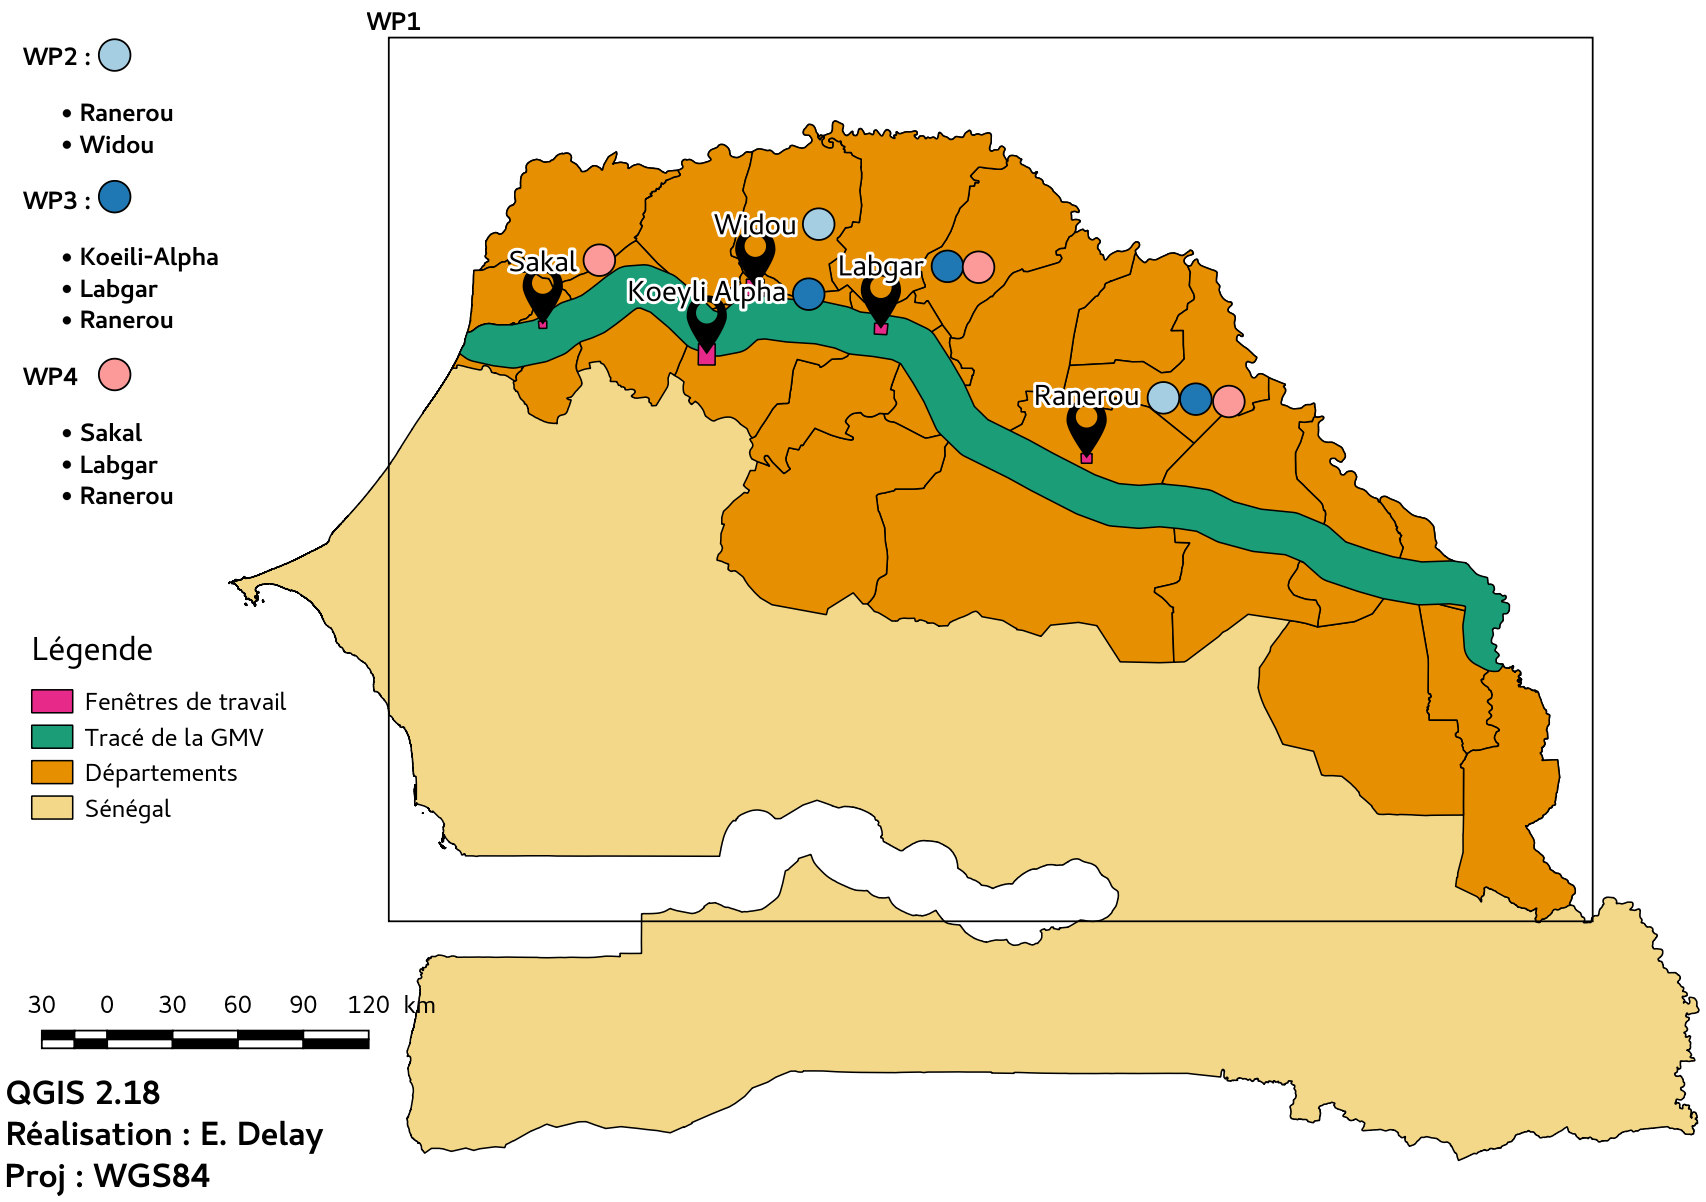
\includegraphics[width = 0.8\textwidth]{img/Carte_FutureSahel}
	\caption{FutureSahel Work Packages}
\end{figure}
\end{frame}

%-=-=-=-=-=-=-=-=-=-=-=-=-=-=-=-=-=-=-=-=-=-=-=-=
%	FRAME: ANR framework in 4 wp
%-=-=-=-=-=-=-=-=-=-=-=-=-=-=-=-=-=-=-=-=-=-=-=-=

\begin{frame}[c]{Focus on WP1}
\vspace{-1cm}
2 goals for WP1 :
\begin{itemize}
	\item In close cooperation with the Senegal agency of Green Great Wall (ANGMV), build a database for researcher and green great wall managers.
	\begin{itemize}
		\item researcher $\rightarrow$ Maintain and exploit data producted in a research context (landscape ecology);
		\item managers $\rightarrow$ use knowlege for spatio-temporel planification.
	\end{itemize}
\end{itemize}
\end{frame}

%-=-=-=-=-=-=-=-=-=-=-=-=-=-=-=-=-=-=-=-=-=-=-=-=
%	FRAME: Goals for our SGBD
%-=-=-=-=-=-=-=-=-=-=-=-=-=-=-=-=-=-=-=-=-=-=-=-=

\begin{frame}[c]{Material and methods}
\vspace{-1cm}
\begin{itemize}
	\item The initial architecure developped on PostgreSQL and PostGIS (GEOLAB);
	\item Stay compatible with BBees metadatas;
	\item We need to find a way to deel with heterogen space and time data :
	\begin{itemize}
		\item Raster (Spot, Modis, Landsat, Sentinel);
		\item statistical information produced by gouvernte;
		\item field data.
	\end{itemize}
	\item Technology transfer to stackolders (ANGMV), we need to choose free and open source software.
\end{itemize}
\begin{figure}
	\centering
	
\includegraphics[height=20mm]{img/PostGIS_logo}
	
\includegraphics[height=20mm]{img/QGis_Logo}
	
\includegraphics[height=20mm]{img/GrassGIS_banner}
	
\includegraphics[height=20mm]{img/Rlogo}
\end{figure}
\end{frame}

%-=-=-=-=-=-=-=-=-=-=-=-=-=-=-=-=-=-=-=-=-=-=-=-=
%	FRAME: context
%-=-=-=-=-=-=-=-=-=-=-=-=-=-=-=-=-=-=-=-=-=-=-=-=

\section{Some results}

%-=-=-=-=-=-=-=-=-=-=-=-=-=-=-=-=-=-=-=-=-=-=-=-=
%	FRAME: WP
%-=-=-=-=-=-=-=-=-=-=-=-=-=-=-=-=-=-=-=-=-=-=-=-=

\begin{frame}[c]WP1 : large scale data}
\vspace{-2em}
\begin{figure}
	\centering
	\includegraphics[width = 8cm]{img/map_france}
\end{figure}
\end{frame}

%-=-=-=-=-=-=-=-=-=-=-=-=-=-=-=-=-=-=-=-=-=-=-=-=
%	FRAME: WP
%-=-=-=-=-=-=-=-=-=-=-=-=-=-=-=-=-=-=-=-=-=-=-=-=

\begin{frame}[c]WP2 : plant biologie and phenologie}
\vspace{-2em}
\begin{figure}
	\centering
	\includegraphics[width = 8cm]{img/map_france}
\end{figure}
\end{frame}

%-=-=-=-=-=-=-=-=-=-=-=-=-=-=-=-=-=-=-=-=-=-=-=-=
%	FRAME: WP
%-=-=-=-=-=-=-=-=-=-=-=-=-=-=-=-=-=-=-=-=-=-=-=-=

\begin{frame}[c]WP3 : Sector exploration and planing}
\vspace{-2em}
\begin{figure}
	\centering
	\includegraphics[width = 8cm]{img/map_france}
\end{figure}
\end{frame}

%-=-=-=-=-=-=-=-=-=-=-=-=-=-=-=-=-=-=-=-=-=-=-=-=
%	FRAME: WP
%-=-=-=-=-=-=-=-=-=-=-=-=-=-=-=-=-=-=-=-=-=-=-=-=

\begin{frame}[c]WP4 : Resiliance}
\vspace{-2em}
\begin{figure}
	\centering
	\includegraphics[width = 8cm]{img/map_france}
\end{figure}
\end{frame}


%-=-=-=-=-=-=-=-=-=-=-=-=-=-=-=-=-=-=-=-=-=-=-=-=
%	FRAME: MERCI DE VOTRE ATTENTION
%-=-=-=-=-=-=-=-=-=-=-=-=-=-=-=-=-=-=-=-=-=-=-=-=
{
\usebackgroundtemplate{
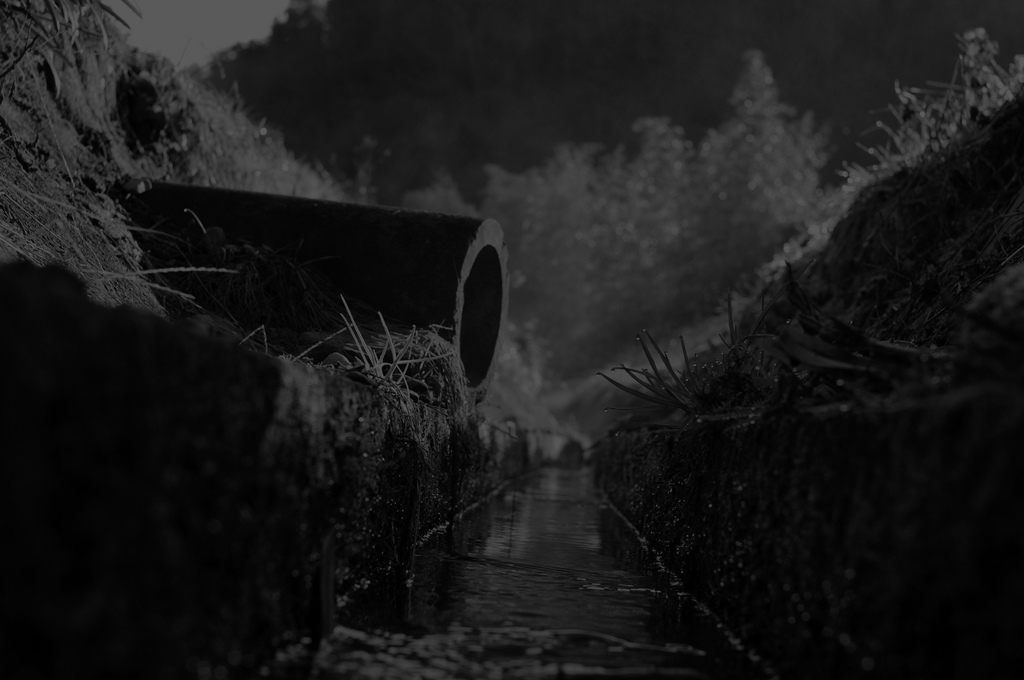
\includegraphics[width=\paperwidth]{img/fin.jpg}}%
\begin{frame}
  \vspace{-1em}
  \begin{minipage}[t][.8\textheight]{\textwidth}
    \color{\cnGrey}{\LARGE{Thank you for your attention}}

    \vfill

  \hfill \small{Photo credit : Thomas m-louis. sur 
\includegraphics[height=0.55cm]{img/flickr_logo}}
  \end{minipage}
  \vspace{-3em}
  \centering
	You can find this presentation on github
\includegraphics[height=0.85cm]{img/github}

\end{frame}
}

%-=-=-=-=-=-=-=-=-=-=-=-=-=-=-=-=-=-=-=-=-=-=-=-=
%	FRAME: ANNEXE PHOTOS
%-=-=-=-=-=-=-=-=-=-=-=-=-=-=-=-=-=-=-=-=-=-=-=-=
{
\usebackgroundtemplate{
\includegraphics[width=\paperwidth]{img/annexe_boulange}}%
\begin{frame}
  \vspace{-1em}
  \begin{minipage}[t][.8\textheight]{\textwidth}
    \color{\cnGrey}{\LARGE{~}}

    \vfill

  \hfill \small{Photo credit : James Linton}
  \end{minipage}

\end{frame}
}

%-=-=-=-=-=-=-=-=-=-=-=-=-=-=-=-=-=-=-=-=-=-=-=-=
{
\usebackgroundtemplate{
\includegraphics[width=\paperwidth]{img/annexe_canal1}}%
\begin{frame}
  \vspace{-1em}
  \begin{minipage}[t][.8\textheight]{\textwidth}
    \color{\cnGrey}{\LARGE{~}}

    \vfill

  \hfill \small{Photo credit : James Linton}
  \end{minipage}

\end{frame}
}

%-=-=-=-=-=-=-=-=-=-=-=-=-=-=-=-=-=-=-=-=-=-=-=-=
{
\usebackgroundtemplate{
\includegraphics[width=\paperwidth]{img/annexe_irrigation}}%
\begin{frame}
  \vspace{-1em}
  \begin{minipage}[t][.8\textheight]{\textwidth}
    \color{\cnGrey}{\LARGE{~}}

    \vfill

  \hfill \small{Photo credit : James Linton}
  \end{minipage}

\end{frame}
}

%-=-=-=-=-=-=-=-=-=-=-=-=-=-=-=-=-=-=-=-=-=-=-=-=
{
\usebackgroundtemplate{
\includegraphics[width=\paperwidth]{img/annexe_old1}}%
\begin{frame}
  \vspace{-1em}
  \begin{minipage}[t][.8\textheight]{\textwidth}
    \color{\cnGrey}{\LARGE{~}}

    \vfill

  \hfill \small{Photo credit : James Linton}
  \end{minipage}

\end{frame}
}

%-=-=-=-=-=-=-=-=-=-=-=-=-=-=-=-=-=-=-=-=-=-=-=-=
{
\usebackgroundtemplate{
\includegraphics[width=\paperwidth]{img/annexe_old2}}%
\begin{frame}
  \vspace{-1em}
  \begin{minipage}[t][.8\textheight]{\textwidth}
    \color{\cnGrey}{\LARGE{~}}

    \vfill

  \hfill \small{Photo credit : James Linton}
  \end{minipage}

\end{frame}
}

%-=-=-=-=-=-=-=-=-=-=-=-=-=-=-=-=-=-=-=-=-=-=-=-=
{
\usebackgroundtemplate{
\includegraphics[width=\paperwidth]{img/annexe_rai}}%
\begin{frame}
  \vspace{-1em}
  \begin{minipage}[t][.8\textheight]{\textwidth}
    \color{\cnGrey}{\LARGE{~}}

    \vfill

  \hfill \small{Photo credit : James Linton}
  \end{minipage}

\end{frame}
}

%-=-=-=-=-=-=-=-=-=-=-=-=-=-=-=-=-=-=-=-=-=-=-=-=
{
\usebackgroundtemplate{
\includegraphics[width=\paperwidth]{img/annexe_vanne}}%
\begin{frame}
  \vspace{-1em}
  \begin{minipage}[t][.8\textheight]{\textwidth}
    \color{\cnGrey}{\LARGE{~}}

    \vfill

  \hfill \small{Photo credit : James Linton}
  \end{minipage}

\end{frame}
}

%-=-=-=-=-=-=-=-=-=-=-=-=-=-=-=-=-=-=-=-=-=-=-=-=
{
\usebackgroundtemplate{
\includegraphics[width=\paperwidth]{img/annexe_verger}}%
\begin{frame}
  \vspace{-1em}
  \begin{minipage}[t][.8\textheight]{\textwidth}
    \color{\cnGrey}{\LARGE{~}}

    \vfill

  \hfill \small{Photo credit : James Linton}
  \end{minipage}

\end{frame}
}


%-=-=-=-=-=-=-=-=-=-=-=-=-=-=-=-=-=-=-=-=-=-=-=-=
%	FRAME: LOACL VISION
%-=-=-=-=-=-=-=-=-=-=-=-=-=-=-=-=-=-=-=-=-=-=-=-=
%
%\begin{frame}[c]{What about Wittfogel ?}
%\begin{alertblock}{\textsc{Note}}
%	\begin{itemize}
%		\item We can consider local politicians as Leon Jean Grégory as the heirs of the hydraulic elite. They try to improve their own vision of modernity.
%		\item Leon Jean Grégory is still in memory and his legacy is maintained by the ASA. Indeed today, this vision is a way to oppose irritants to the water agency.
%		\item underlines the shift from a policy of demand to supply policy
%	\end{itemize}
%\end{alertblock}
%\end{frame}
%
%%-=-=-=-=-=-=-=-=-=-=-=-=-=-=-=-=-=-=-=-=-=-=-=-=
%%	FRAME: LOACL VISION
%%-=-=-=-=-=-=-=-=-=-=-=-=-=-=-=-=-=-=-=-=-=-=-=-=
%
%\begin{frame}[c]{What about Wittfogel ?}
%\begin{alertblock}{\textsc{Note}}
%	\begin{itemize}
%		\item We can consider local politicians as Leon Jean Grégory as the heirs of the hydraulic elite. They try to improve their own vision of modernity.
%		\item Leon Jean Grégory is still in memory and his legacy is maintained by the ASA. Indeed today, this vision is a way to oppose irritants to the water agency.
%		\item underlines the shift from a policy of demand to supply policy
%	\end{itemize}
%\end{alertblock}
%\end{frame}
%
%%-=-=-=-=-=-=-=-=-=-=-=-=-=-=-=-=-=-=-=-=-=-=-=-=
%%	FRAME: Simplicity in complexity
%%-=-=-=-=-=-=-=-=-=-=-=-=-=-=-=-=-=-=-=-=-=-=-=-=
%%\section{Simplicity in complexity}
%\section{Death by certainty}
%
%%-=-=-=-=-=-=-=-=-=-=-=-=-=-=-=-=-=-=-=-=-=-=-=-=
%%	FRAME: CHANGES
%%-=-=-=-=-=-=-=-=-=-=-=-=-=-=-=-=-=-=-=-=-=-=-=-=
%\begin{frame}[c]{Change in perspective}
%however, a more complex set of dialectical relations is at play in this situation, requiring a subtler explanatory tool.
%	\begin{block}{\textsc{hypotheses}}
%	\begin{itemize}
%		\item We show that the dam has had the effect of transferring expertise and social power from local to central authority, but not in a direct way.
%		\item Rather, the production of hydrological certainty in the form of assured and regular flows has weakened the local social structures and relations that had evolved to accommodate - and were sustained by - hydrological uncertainty and periodical scarcity
%	\end{itemize}
%	\end{block}
%\end{frame}
%
%%-=-=-=-=-=-=-=-=-=-=-=-=-=-=-=-=-=-=-=-=-=-=-=-=
%%	FRAME: Technological Changes
%%-=-=-=-=-=-=-=-=-=-=-=-=-=-=-=-=-=-=-=-=-=-=-=-=
%\begin{frame}[c]{Technological Changes}
%	\begin{block}{\textsc{Facts}}
%		dam is filling its two main tasks : irrigation and reducing flood peaks
%	\end{block}
%	\begin{itemize}
%		\item shift of gravity irrigation to pressurized irrigation
%		\item gravity irrigation :
%			\begin{itemize}
%				\item role of socio-spatial entropy reduction
%			\end{itemize}
%		\item pressurized irrigation
%			\begin{itemize}
%				\item expand irrigated areas (at constant volume)
%				\item regroup plots more easily
%				\item reduce the arduous nature of irrigation (automatization)
%			\end{itemize}
%	\end{itemize}
%\end{frame}
%
%%-=-=-=-=-=-=-=-=-=-=-=-=-=-=-=-=-=-=-=-=-=-=-=-=
%%	FRAME: what have we to lost
%%-=-=-=-=-=-=-=-=-=-=-=-=-=-=-=-=-=-=-=-=-=-=-=-=
%\begin{frame}[c]{What have we lost}
%	\begin{itemize}
%		\item It provokes a vertical shift of responsibility
%		\begin{itemize}
%			\item historical responsibility was linked to the neighbors
%			\item today is being linked to ASA administrators
%		\end{itemize}
%		\item Canals had a responsibility the recharging of aquifers, it question the Leon Jean Grégory legacy.
%	\end{itemize}
%\end{frame}

%-=-=-=-=-=-=-=-=-=-=-=-=-=-=-=-=-=-=-=-=-=-=-=-=
%	FRAME: The hydrosocial cycle
%-=-=-=-=-=-=-=-=-=-=-=-=-=-=-=-=-=-=-=-=-=-=-=-=
\begin{frame}[c]{The hydro social cycle}
	\vspace{-2em}
	We employ the concept of the hydro social cycle  - which borrows from Wittfogel's dialectic, but demands a more complex account of hydro social relations -- to explain these developments.
	\begin{figure}
	\vspace{-1em}
	\centering
	\includegraphics[width = 0.8\textwidth]{img/hydrosocial_cycle}
	 \caption{hydrosocial cycle}
\end{figure}

\end{frame}

%%-=-=-=-=-=-=-=-=-=-=-=-=-=-=-=-=-=-=-=-=-=-=-=-=
%%
%%	SECTION: CONCLUSION
%%
%%-=-=-=-=-=-=-=-=-=-=-=-=-=-=-=-=-=-=-=-=-=-=-=-=
%\section*{Conclusion}
%
%%-=-=-=-=-=-=-=-=-=-=-=-=-=-=-=-=-=-=-=-=-=-=-=-=
%%	FRAME:
%%-=-=-=-=-=-=-=-=-=-=-=-=-=-=-=-=-=-=-=-=-=-=-=-=
%
%\begin{frame}[c]{Conclusion}
%\vspace{-2em}
%\begin{exampleblock}{Our hypothesizing}
%	Some of the longer-term consequences of the dam in terms of its unintended impacts on the agricultural sector of the region and, ultimately, on the influence of the state.
%\end{exampleblock}
%
%\end{frame}


\end{document}
